\documentclass[10pt,norsk,a4paper]{article}
\usepackage[utf8]{inputenc}
\usepackage[T1]{fontenc}
\usepackage[norsk]{babel}
\usepackage[cm]{fullpage}
\usepackage{color}
\usepackage{parskip,textcomp,amssymb,graphicx}
\usepackage{pdfpages}
\usepackage[stable]{footmisc}
\usepackage{multicol}


\title{Generalforsamling \\
	Høst 2018\\[3cm]
	
\includegraphics[width=3cm,trim=0 4cm 0 0]{../../res/logo.png}\\}
\date{21.\ november 2018}
\author{Ifi-dagen}

% Blank header, samt footer med side x av y
\usepackage{fancyhdr}
\pagestyle{fancy}
\renewcommand{\headrulewidth}{0pt}
\fancyhead{}
\cfoot{Side~\thepage\ av~\pageref{lastpage}}


\begin{document}

\maketitle{}
\newpage
\part{Dagsorden og detaljer}
\tableofcontents{}
\newpage


\section{Valg av møteleder}

\section{Valg av referent}

\section{Valg av protokollunderskrivere}

\section{Valg av tellekorps}

\section{Godkjenning av innkalling}

\section{Godkjenning av dagsorden}

\section{Årsberetning v/ leder}
Til utfylling.

\section{Regnskap og revidert budsjett}
Økonomiansvarlig orienterer.

\subsection{Regnskap for 2018}
Økonomiansvarlig legger fram regnskapsresultatet for 2018.

\subsection{Budsjett for 2019}
Økonomiansvarlig legger fram tentativt forslag til budsjett for 2019.

\section{Valg}
\subsection{Leder}
\subsection{Nestleder}
\subsection{Økonomiansvarlig}
\subsection{Bedriftsansvarlig}
\subsection{Faglig ansvarlig}
\subsection{Funksjonæransvarlig}
\subsection{Promoteringsansvarlig}
\subsection{Teknisk ansvarlig}
\subsection{Underholdningsansvarlig}

\section{Vedtektsendringer}
Eventuelle vedtektsendringer vil legges til her.\label{lastpage}

\newpage
\part{Nåværende vedtekter}
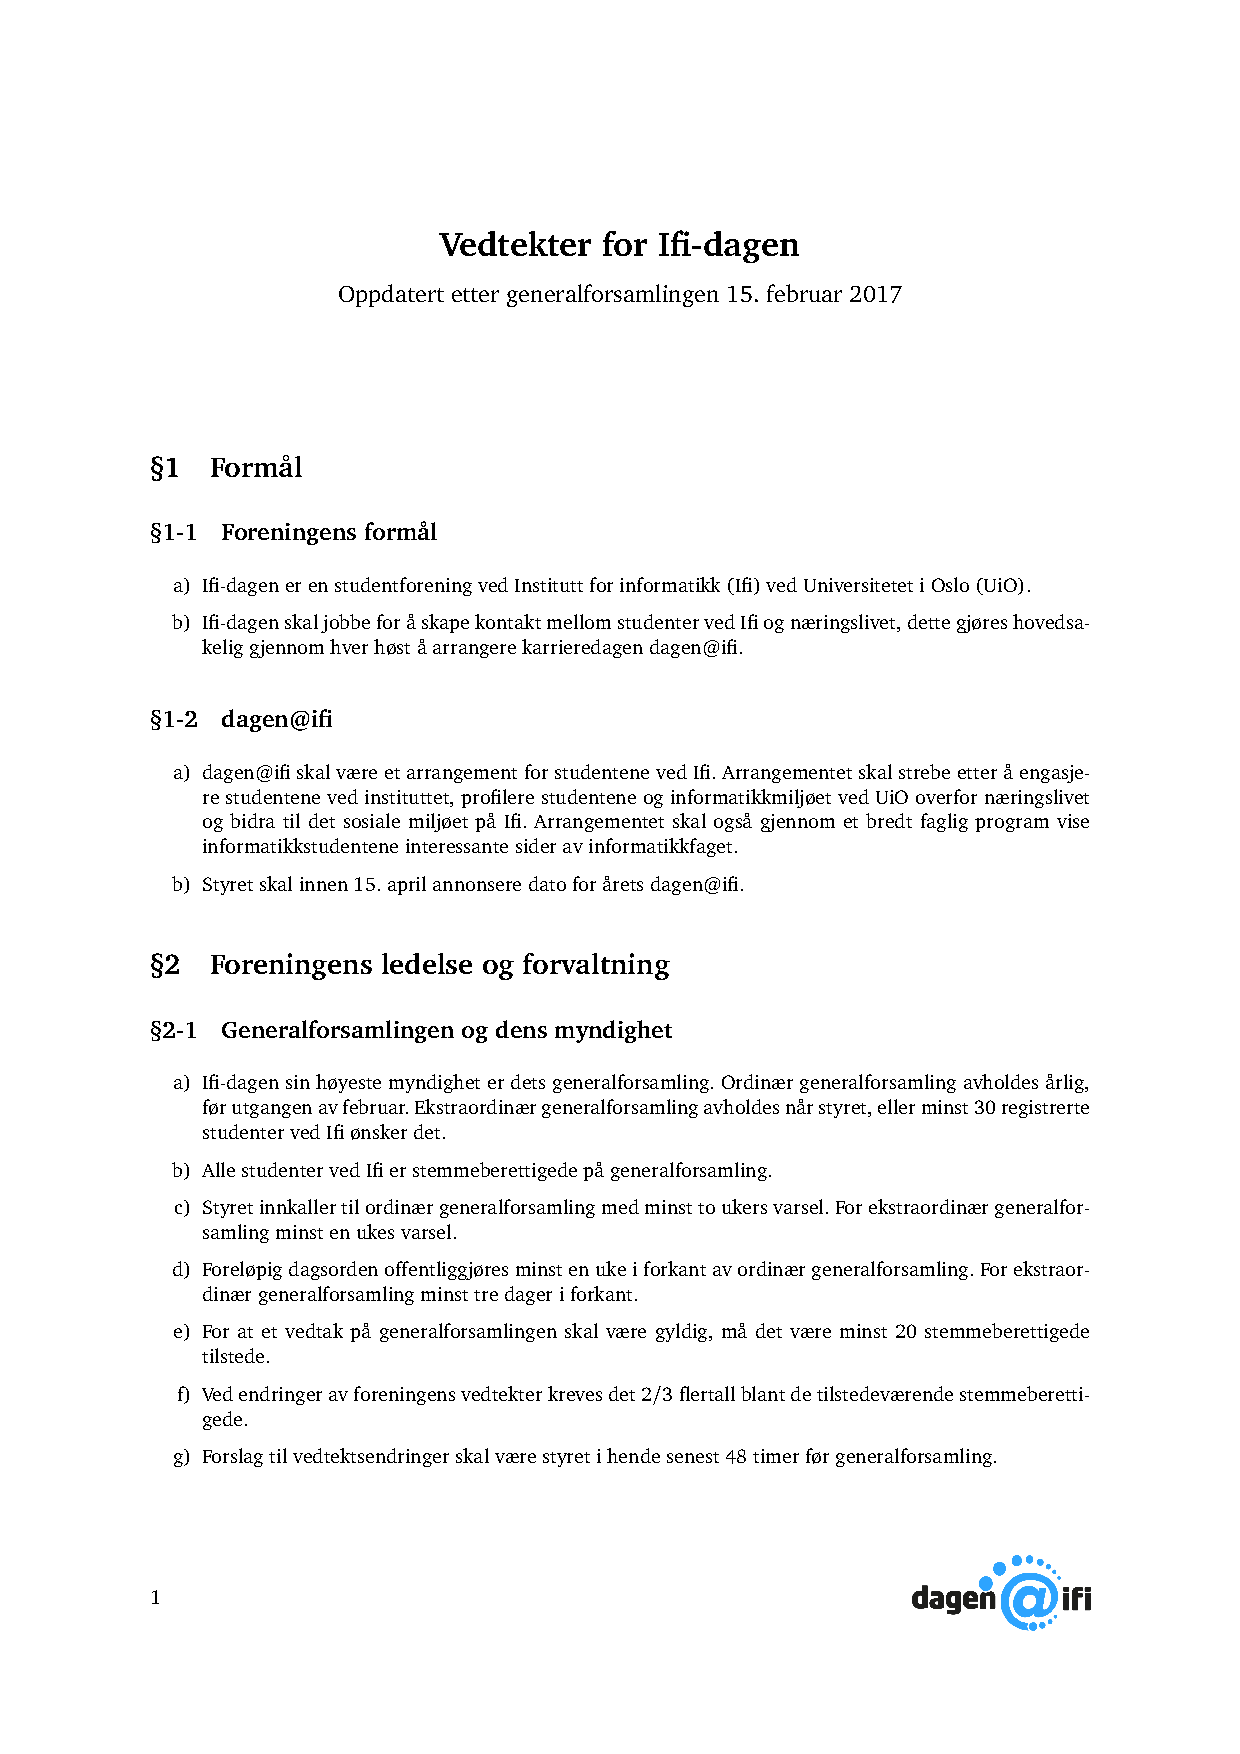
\includepdf[pages=-]{../../vedtekter/vedtekter.pdf}
\end{document}
